\documentclass{beamer}
\usetheme[sectionpage=none]{metropolis}
%\usepackage{booktabs} 
\usepackage{url}
\def\UrlBreaks{\do\/\do-}
\usepackage{amsfonts, amsmath, lmodern}
\usefonttheme{serif}
\usepackage{algorithm}
\usepackage{algorithmic}
\usepackage[ngerman]{babel}
\usepackage{bm}


%plots
\usepackage{tikz}
\usepackage{pgfplots}
\usepackage{pgfplotstable}
\pgfplotsset{compat=newest}
\usepackage{subcaption}
\usepackage{csvsimple}

%bibliography numbers
\setbeamertemplate{bibliography item}{\insertbiblabel}

\graphicspath{{./pictures_eps}}





\title{Fast Search of the Optimal Contraction Sequence in Tensor Networks\cite{9325533}}

\author{Max Koch, Christian Ortlepp}

\institute{Friedrich-Schiller-Universität Jena}

\date{20. Januar 2023}



\begin{document}
	
	\maketitle 
	\begin{frame}{Gliederung}
		\tableofcontents
	\end{frame}
	
	\begin{section}{Evaluationsmetriken}
		\begin{frame}{Unterschiedliche Evaluationsmetriken}
			\begin{columns}[]

				\column{.5\textwidth}
					\textbf{Total Contraction Expense (TCE)}
					\begin{itemize}
						\item Summe aller Speicher- bzw. Rechenkosten einer Kontraktionsreihenfolge
					\end{itemize}
					\begin{align*}
						e_1 &= 10, e_2 = 20, e_3 = 30 \\
						&\rightarrow E_{total} = 60
					\end{align*}


				\column{.5\textwidth}
					\textbf{Maximum Contraction Expense (MCE)}
					\begin{itemize}
						\item Maximum der Kosten einer Kontraktion in einer Kontraktionsreihenfolge
					\end{itemize}
					\begin{align*}
						e_1 &= 10, e_2 = 20, e_3 = 30 \\
						&\rightarrow E_{max} = 30
					\end{align*}
			\end{columns}
		\end{frame}

		\begin{frame}{Unterschiedliche Evaluationsmetriken}
			\begin{columns}	
				\column{.5\textwidth}
						\textbf{Total Contraction Expense (TCE)}
						\begin{itemize}
							\item genauer als nur das Maximum zu bestimmen
							\item langsamer
						\end{itemize}


				\column{.5\textwidth}
					\textbf{Maximum Contraction Expense (MCE)}
					\begin{itemize}
						\item falls die Dimensionen der Tensoren groß sind, ist die Differenz zwischen der TCE und der MCE gering
						\item durch effizienteres Caching schneller in Hardware umsetzbar
					\end{itemize}

			\end{columns}
		\end{frame}

		\begin{frame}{Unterschiedliche Evaluationsmetriken}
			\textbf{$\rightarrow$ maximum contraction expense wird verwendet}
			\begin{align*}
				MS &= \max_t SE(sq_t)\\ MC &= \max_t CE(sq_t)
			\end{align*}
			% nur ein Beispiel
			Beispiel für eine Kontraktionsreihenfolge:
			$sq = ((((\bm{\tau}_{1} \bm{\tau}_{4}) \bm{\tau}_{2}) \bm{\tau}_{3}) \bm{\tau}_{1})$
		\end{frame}

	\end{section}

	\begin{section}{Beispielkontraktionen und Beispielberechnungen}
	
		\begin{frame}{Beispielkontraktionen und Berechnung von MC/MS}
			\begin{figure}
				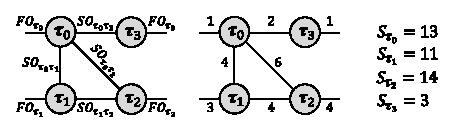
\includegraphics{figure_03_a}
				\caption{beliebiges Netzwerk mit angegebenen free/sharing orders}
			\end{figure}
		\end{frame}

		\begin{frame}{Beispielkontraktionen und Berechnung von MC/MS}
			\begin{figure}
				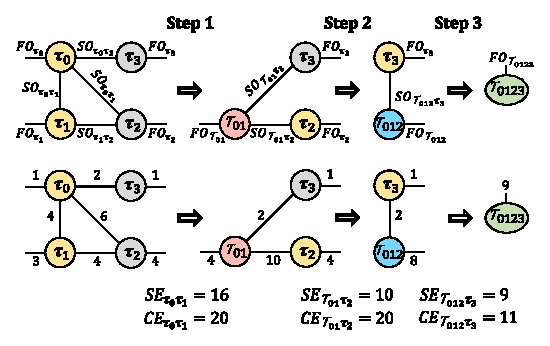
\includegraphics{figure_03_b}
				\caption{beliebige Kontraktion mit Angabe des jeweiligen SE und CE}
			\end{figure}
		\end{frame}

		\begin{frame}{Beispielkontraktionen und Berechnung von MC/MS}
			\begin{figure}
				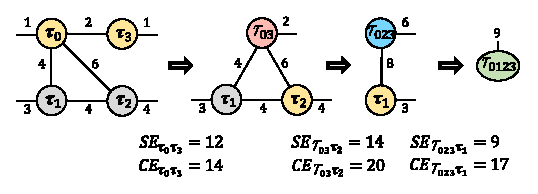
\includegraphics{figure_03_c}
				\caption{Kontraktion mit bestmöglichem MS}
			\end{figure}
		\end{frame}

		\begin{frame}{Beispielkontraktionen und Berechnung von MC/MS}
			\begin{figure}
				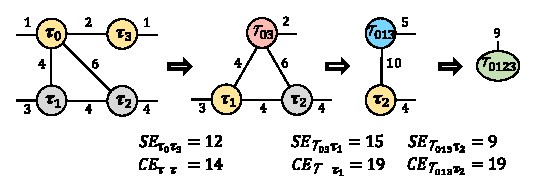
\includegraphics{figure_03_d}
				\caption{Kontraktion mit bestmöglichem MC}
			\end{figure}
		\end{frame}

		\begin{frame}{Beispielkontraktionen und Berechnung von MC/MS}
			\begin{align*}
				sq_{MS} &= (((\bm{\tau}_{0} \bm{\tau}_{3}) \bm{\tau}_{2}) \bm{\tau}_{1}) \\
				sq_{MC} &= (((\bm{\tau}_{0} \bm{\tau}_{3}) \bm{\tau}_{1}) \bm{\tau}_{2})
			\end{align*}
			\begin{equation*}
				\rightarrow sq_{MS} \neq sq_{MC}
			\end{equation*}
			\begin{itemize}
				\item die Kontraktionsreihenfolgen für den kleinsten Speicher- bzw. Rechenaufwand sind nicht zwangsläufig identisch
				\item es muss entschieden werden, was optimiert werden soll
			\end{itemize}
		\end{frame}

	\end{section}

	\begin{section}{$Set_v$ und $Split_v$}

		\begin{frame}{$Set_v$ und $Split_v$}
			\begin{itemize}
				\item $Set_v$ ist die Menge aller möglichen Tensoren, welche aus $v$ ursprünglichen Tensoren kontrahiert wurden in einem Netzwerk mit $V$ Tensoren
				\item für $V = 3$ ist $Set_2 = \{\bm{T}_{01}, \bm{T_}{02}, \bm{T}_{12} \}$ und $Set_3 = \{\bm{T}_{012} \}$
			\end{itemize}
		\end{frame}

		\begin{frame}{$Set_v$ und $Split_v$}
			\begin{itemize}
				\item jeder Tensor aus $Set_v$ kann auf $Split_v$ verschiedene Arten in einem Schritt aus zwei verschiedenen Teiltensoren kontrahiert werden
				\item der Tensor $\bm{T}_{012} \in Set_3$ kann kontrahiert werden aus $\{\bm{\tau}_0, \bm{T}_{02} \}$, $\{\bm{\tau}_{1}, \bm{T}_{02} \}$ oder $\{\bm{\tau}_{2}, \bm{T}_{01} \}$ $\rightarrow Split_3 = 3$
			\end{itemize}
			\begin{align*}
				Split_v &= \begin{cases}
					\sum^{\lfloor v/2 \rfloor}_{k=1} \binom{v}{k} &\text{falls v ungerade} \\
					\sum^{\lfloor v/2 \rfloor}_{k=1} \binom{v}{k} + \frac{\binom{v}{v/2}}{2} & \text{falls v gerade}
				\end{cases} \\
				&= \frac{2^v - 2}{2} = \mathcal{O}(2^v)
			\end{align*}
		\end{frame}

	\end{section}
	
	
	
	
	
	\begin{frame}[allowframebreaks]{Bibliography}
		\bibliography{../bibliography/bibliography.bib}
		\bibliographystyle{splncs04}
	\end{frame}
	
\end{document}
